

\section{Grundlagen}
Im diesem erste Kapitel sollen die Grundlagen, die für diese Arbeit als Wichtig empfunden wurde, aufgelistet werden. Das Hauptaugenmerk wird dabei auf die beiden Steuerverfahren, Phasenanschnitt- und Schwingungspaketsteuerung, sowie auf deren Vor- \& Nachteile gerichtet. Da bei solchen Methoden das auftreten von verzerrten Signalen fast nicht zu vermeiden ist, enthält der folgende Abschnitt einige Details über das Vorkommen und die Auswirkungen von Ober-, Zwischen und Subharmonischen Schwingungen. Durch Normen welche zwingend eingehalten werden müssen, sind bei den beiden Verfahren gewisse Grenzen gesetzt. Damit man versteht auf welche Normen geachtete wurde, sind schlussendlich die drei wichtigsten zusammengefasst.      

\subsection{Auftretende von verzerrten Sinusschwingungen}
Im Idealfall würde bei einer Stromversorgung überall eine perfekte sinusförmige Spannung vorliegen. Jedoch sieht dies in der Realität anders aus. Die Kurve der Spannung und des Stromes weichen massiv von einer Sinusfunktion ab. Man bezeichnet diese verzerrten Schwingungsformen im Allgemeinen als oberschwingungsbehaftetes Signal. \\
Schon früh erkannte man diese Oberschwingungsverzerrungen am Netz, jedoch ist es erst heute ein ernstzunehmendes Problem für die Versorgungsbetriebe, die Verteilnetzbetreiber und für den Endkunden. Früher waren die grössten Herausforderungen, die Auswirkungen von Oberschwingungsverzerrungen auf elektrische Maschinen zu erkennen. Man stellte ausserdem fest, dass Störungen in den Telefonleitungen auftraten, welche den Ton der Sprache beeinträchtigte. Allerdings kann man sagen, dass Oberschwingungsverzerrungen früher ein geringeres Gefahrenpotential darstellten als heute. Die heutigen Maschinen wurden neuerdings so konstruiert, dass sie weniger Oberwellen erzeugen. Auch bei den Verteilnetzen wurde darauf geachtet, dass sie nicht mehr an der Lastobergrenze arbeiten und so ein reineres Sinussignal verwenden. Seit einigen Jahren steigt, die weltweite Nachfrage nach energieeffizienten Lösungen, die nur über vermehrten Einsatz von Leistungselektronik realisierbar sind. 
\subsection{Oberschwingungen}
Die Bedeutung Oberschwingung kommt aus dem Themenbereich «physische Eigenwertprobleme» also Wellen, deren Frequenz ganzzahlige Vielfache der Grundschwingungen sind. In der Musikwelt kann man Oberschwingungsfrequenzen vor allem bei Saiteninstrumenten, wie zum Beispiel bei einer Gitarre oder einer Geige beobachten.\\
Die meisten elektrischen Geräte halten nach der perfekten Welle Ausschau. Bei Wechselstrom definiert die Perfektion eine perfekte Sinuskurve. Die daraus verwendete elektrische Spannung wechselt gleichmässig zwischen der positiven un negativen Halbwelle hin und her. Bei einer Frequenz von \SI{50}{Hz} beträgt dies genau 50-mal pro Sekunde. Der Begriff Welle ist mit dem Zusammenhang von Oberschwingungen nicht ganz korrekt. Eine Welle hat eine räumliche und zeitliche Ausdehnung, jedoch haben die hier betrachteten Schwingungen nur eine zeitliche Ausdehnung. Die Oberschwingungsanteile in einem Wechselstromsystem sind also definiert als sinusförmige Anteile einer periodischen Schwingung, deren Frequenz einem ganzzahligen Vielfachen (Ordnungszahl) der Grundfrequenz entspricht. In der unteren Tabelle \ref{tab:Oberschwingungfrequenz} erkennt man, welche Ordnungszahl $(n)$  zu welcher Frequenz $(fh)$ gehört. Es ist ersichtlich, dass zum Beispiel die 5. Oberschwingung eine Frequenz von \SI{250}{Hz} hat. Die Berechnung der Oberschwingungsfrequenz ist in der unterstehenden Formel \ref{eq:Oberschwingungsfrequenz} dargestellt.

\newpage
\begin{equation}\label{eq:Oberschwingungsfrequenz}
f_h = n \cdot Grundfrequenz
\end{equation}

\begin{table}[ht!]
	
	\centering
	
	\begin{tabular}{|l|l|}
		
		\hline
		
		\begin{tabular}[c]{@{}l@{}}Ordnungszahl\\   $n$\end{tabular} & \begin{tabular}[c]{@{}l@{}}Oberschwingungs-\\frequenz (Hz)  $f_h$\end{tabular} \\ \hline
		
		1                                                            & 50                                                              \\ \hline
		
		3                                                            & 150                                                             \\ \hline
		
		5                                                            & 250                                                             \\ \hline
		
		7                                                            & 350                                                             \\ \hline
		
		11                                                           & 550                                                             \\ \hline
		
		13                                                           & 650                                                             \\ \hline
		
		…                                                            & …                                                               \\ \hline
		
		n                                                            & 50*n                                                            \\ \hline
		
	\end{tabular}
	
	\caption{Oberschwingungsfrequenzen}\label{tab:Oberschwingungfrequenz}
	
\end{table}

Die folgenden zwei Abbildungen \ref{fig:Schwing3} \& \ref{fig:Schwing11} zeigen eine Grundschwingung bei 50 Hz (blau) und die jeweilige 3. und 11. Ordnung der Grundfrequenz (gelb).

\begin{figure}[ht!]
	\begin{minipage}[t]{0.49\textwidth}
		\centering
		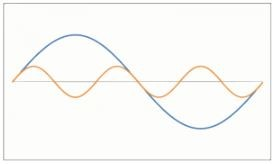
\includegraphics[scale=2]{Schwing_3.jpg}	
		\caption{Grundschwingung mit 3. Ordnung \cite{Oberwellen}}\label{fig:Schwing3}
	\end{minipage}	
	%
	\begin{minipage}[t]{0.49\textwidth}	
		\centering	
		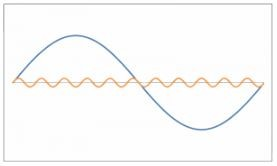
\includegraphics[scale=2]{Schwing_11.jpg}	
		\caption{Grundschwingung mit 11. Ordnung \cite{Oberwellen}}\label{fig:Schwing11}
	\end{minipage}
\end{figure}



\subsection{Verzerrte Schwingung}\label{sec:Verzerrte_Schwingung}
Eine verzerrte Schwingung entsteht durch Überlagerungen von verschiedenen sinusförmigen Wellen mit unterschiedlichen Frequenzen und Amplituden. Man kann eine solche Schwingung mit den unterschiedlichen Oberschwingungskomponenten zusammensetzen, indem man eine Sinusschwingung mit mehreren Oberschwingungen zusammenaddiert. Ein wellenförmiges verzerrtes Signal lässt sich so zu einer Grundschwingung mit ihren mehreren harmonischen Oberschwingungen zerlegen. Bei der untenstehenden Graphik \ref{fig:Addition Oberwellen} ist diese ersichtlich, wobei die rote Kurve das verzerrte Signal darstellt. Die drei blauen Sinusschwingungen sind die Zerlegungen zur Grundschwingung, zur 3. und 5. harmonische Oberschwingung. Addiert man die drei blauen Kurven zusammen, so erhält man wiederum das verzerrte rote Signal.
\newpage
\begin{figure}[ht!]
	\centering
	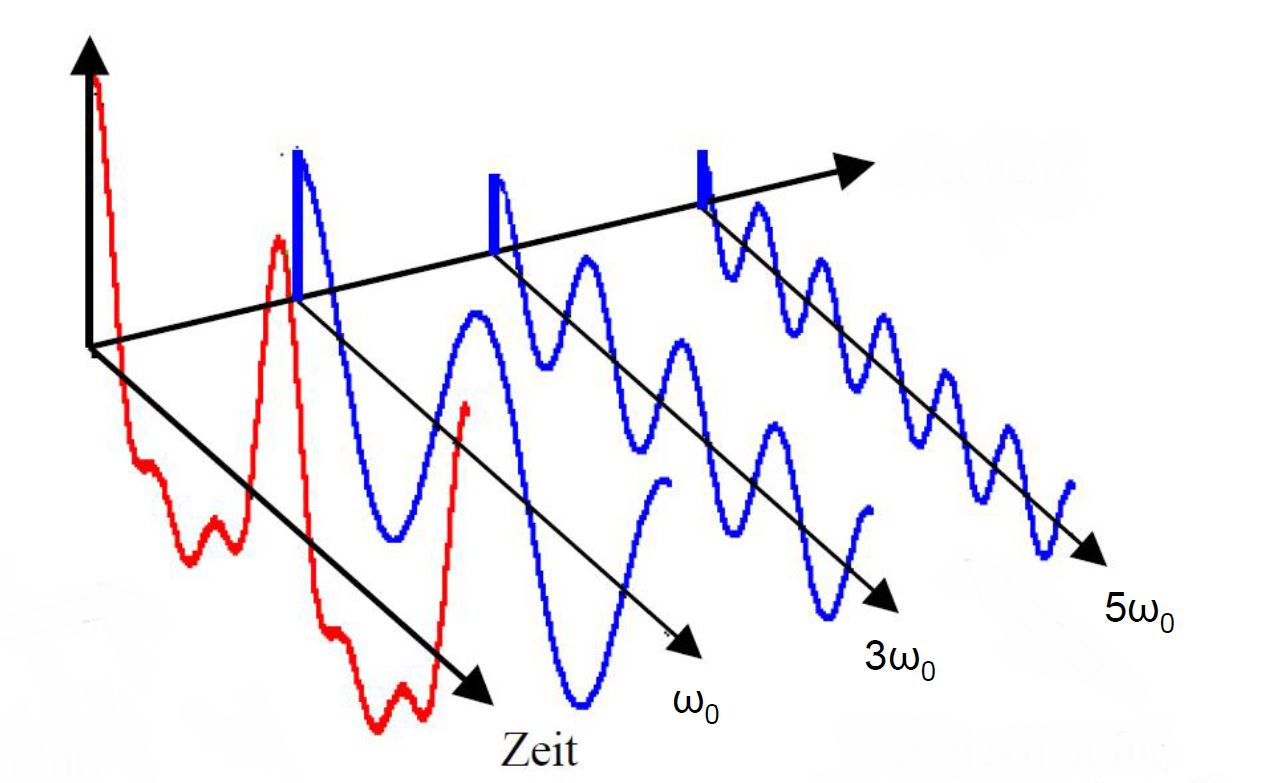
\includegraphics[scale=0.7]{verzerrtes_Signal_analysis.png}	
	\caption{Addition der verschiedenen Oberwellen \cite{analysi3}}\label{fig:Addition Oberwellen}
\end{figure}

Noch heute trägt die Fourier-Transformation dessen Namen. Anhand eines Amplitudenspektrums lassen sich die Sinuskurven bei den verschiedenen harmonischen Frequenzen übersichtlich visualisieren. Da das Amplitudenspektrum jedoch keine Informationen über die Phasenlage der einzelnen Harmonischen enthält wird zusätzlich noch ein Phasenspektrum betrachtet. In der Praxis wird dieses Spektrum jedoch oft einfach weggelassen. Mit der folgenden Fourier-Reihe lässt sich eine beliebige periodische Funktion als Summe von Sinus- und Cosinus-Funktionen darstellen:

\begin{equation}
f(x) = {\frac{a\textsubscript{0}}{2}}+\sum_{n=1}^\infty[a\textsubscript{n} \cdot cos(nx)+b\textsubscript{n} \cdot sin(nx)]
\end{equation}


Mathematisch berechnet man die dazu benötigten Fourier-Koeffizienten $a\textsubscript{0}$, $a\textsubscript{n}$ und $b\textsubscript{n}$ mit Hilfe der untenstehenden Formeln.

\begin{equation}
a\textsubscript{0} =  {\frac{1}{2\pi} \cdot \int_{0}^{2\pi} f(x) dx}
\end{equation}

\begin{equation}
a\textsubscript{n} =  {\frac{1}{\pi} \cdot \int_{0}^{2\pi} f(x) \cdot cos(n \cdot w0 \cdot x) dx}
\end{equation}

\begin{equation}
b\textsubscript{n} =  {\frac{1}{\pi} \cdot \int_{0}^{2\pi} f(x) \cdot sin(n \cdot w0 \cdot x) dx}
\end{equation}

Mit den oben genannten Fourier-Koeffizienten lassen sich nun das Amplituden- und Phasenspektrum berechnen.

\begin{equation}
A\textsubscript{n} = {\sqrt{a\textsubscript{n}^2+b\textsubscript{n}^2}}
\end{equation}

\begin{equation}
\varphi = \arctan\left( \frac{a\textsubscript{n}}{b\textsubscript{n}}\right) 
\end{equation}

Bei den Oberschwingungen gibt es ungerade oder gerade harmonische Schwingungen.
Die ungeraden Oberwellen sind die charakteristischen Oberschwingungsanteile in den heutigen Stromversorgungsnetzen. Sie stellen Wellenformen dar, die bezogen auf die Zeitachse symmetrisch sind. Aufgrund der meist dreiphasigen Symmetrie der heutigen Infrastrukturen sind nahezu alle Signale symmetrisch, obwohl es zu Verzerrung kommt. Geradzahlige Oberschwingungen können nur aus Wellenformen entstehen, die nicht symmetrisch bezogen auf die Zeitachse sind.

\subsection{Vorkommen der Oberschwingungen}
Oberschwingungsströme erzeugt fast jedes elektrische Gerät. Ein wichtiger Bezugspunkt zu den individuellen Oberschwingungsgrössen ist die gesamte harmonische Verzerrung. Man nennt ihn auch den THD-Wert (Total Harmonic Distortion). Diesen Wert gilt es besonders zu verstehen, damit man ihn rechnerisch analysieren kann. Er gibt das Verhältnis des Effektivwertes aller Oberschwingungen zum Effektivwert der Grundschwingung an. Man verwendet ihn üblicherweise im Nieder-, Mittel-, aber auch im Hochspannungsnetz. Normalerweise wird die Verzerrung des Stromes als $THDi$, beschrieben in der Formel \ref{eq:THDi} und die Verzerrung der Spannung als $THDu$, ersichtlich in der Formel \ref{eq:THDu}, angegeben. Der Total Harmonic Current $THC$ ist der gesamte Oberschwingungsstrom. Er wird verwendet, um den Gesamteffektivwert der Oberschwingungsströme der Ordnung 2 bis 40 zu quantifizieren, die zu einer Verzerrung der Stromkurve beitragen. Man erkennt dies in der Formel \ref{eq:THC}. Diesen Wert braucht man vor allem, um die erforderlichen Eigenschaften zur Auswahl eines effizienten aktiven Oberschwingungsfilters zu bestimmen.

\begin{equation}\label{eq:THC}
THC = {\sqrt{\sum_{n=2}^{40} I_n^2}}
\end{equation}



Die gesamte harmonische Verzerrung des Stromes gibt, wie der Name schon sagt, die gesamte Verzerrung des Stromes an. Der Wert ist definiert als Quotient des Effektivwerts der Oberschwingungsströme im Verhältnis zum Grundschwingungsstrom. Typischerweise wird die Summe aller Stromoberschwingungsanteile in Bezug auf den Grundschwingungsstrom bis einschliesslich der 40. Oberschwingung berechnet. Die Oberschwingungsströme, welche durch Lasten in Netzwerken erzeugt werden, müssen durch die Impedanzen der Transformatoren oder Drosseln fliessen. An diesen Impedanzen kommt es zu nichtlinearen Spannungsabfällen. Es werden Oberschwingungsspannungen erzeugt die im ganzen Netz verbreitet werden. Diese können an Endgeräten eine Verzerrung der Versorgungsspannung verursachen. Somit ist die harmonische Verzerrung des Stromes $THDi$ eine direkte Ursache für die Verzerrung der Spannung $THDu$ .Sie gibt das Ausmass der Verzerrung der Versorgungsspannung an. Auch dieser Wert ist definiert als Quotient des Effektivwertes der Spannungsoberschwingungsanteile bis zur 40. Oberschwingung bezogen auf den Effektivwert der Grundschwingung. 
Folgende Formel zeigt, wie die Totale Verzerrung des Stromes in Prozent berechnet ist.
\begin{equation}\label{eq:THDi}
THDi = \frac{\sqrt{\sum_{n=2}^{40} I_n^2}}{I_{(1)}} \cdot 100 \%
\end{equation}

Parallel dazu zeigt die untere Formel die Totale Verzerrung der Spannung in Prozent.
\begin{equation}\label{eq:THDu}
THDu = \frac{\sqrt{\sum_{n=2}^{40} U_n^2}}{U_{(1)}} \cdot 100\%
\end{equation}






Je niedriger der THDu-Wert ist, desto besser ist die Spannungsqualität. Die Norm besagt, dass der gesamte Oberschwingungsgehalt den Wert von 8\% nicht überschreiten darf. Dazu kommt, dass heute üblicherweise für die Verzerrung die THD-Werte angegeben sind und nicht wie früher die Oberschwingungsgehalte (Klirrfaktore).\\
Wenn man sich mit den Oberschwingungsproblematik befasst, ist es wichtig, den Zusammenhang zwischen Strom und Spannung zu verstehen. Dadurch ist es möglich eine geeignete Lösung für das reduzieren von Oberschwingungen zu finden. 
Je nach Eigenschaft der Oberschwingungserzeuger und der Eigenschaft eines Gerätes am elektrischen Netz, verbreiten sich Oberschwingungsströme in einem System unterschiedlich. Verschiedene Spannungsverzerrungen sind die Folgen. 

\subsection{Auswirkung von Oberschwingungen}

Falls Oberschwingungen oder andere Netzrückwirkungen bei Betriebsmitteln auftreten, können die Funktionen von den Geräten beeinträchtigt oder sogar zerstört werden. Ein Beispiel dafür wäre, im Falle einer Kurzzeitunterberechnung bei Schaltnetzteile, würden sie mit extrem hohen Einschaltspitzen reagieren. Diese Spitzen könnten das 20-fache der Nennlast erreichen. Im einphasigen Verbrauch in einem Dreiphasigen-Wechselstromsystem fliesst der ganze Rückleitstrom über den Sternpunkt des Transformators zurück. Gäbe es viele Schaltnetzteile in einem System, würden sich die Rückleiterströme nicht mehr aufheben, sondern sie würden sich addieren. Die Folgen davon wäre eine Sternpunktverschiebung. Oberschwingungen können bei Glühbirnen die Glühfadentemperatur erhöhen und somit die Lebensdauer verkürzen. Auch bei Dreh- oder Wechselstrommotoren und -generatoren führen Stromoberschwingungen zu zusätzlicher Erwärmung. Bei Schutzgeräten wie Distanzschutz, Überstromschutz oder Differentialschutz können Oberschwingungen den Aufbau und die Wirkungswiese des Schutzgerätes beeinflussen. Sind die Abstände zwischen Freileitungen und Telefonleitungen zu gering, können die Oberschwingungen die Sprachübertragung stören. Dabei gibt es vor allem ein Auge auf die 20. bis zur 30. Ordnung der Oberschwingung zu werfen.

\subsection{Zwischen- und Subharmonischen Schwingungen}

Die Subharmonischen sind Sinusförmige Schwingungen, deren Frequenz unterhalb der Grundfrequenz entstehen. Ein Beispiel dafür wären Schwingungen bei Frequenzen von 5, 10, oder 20 Hz bei einer Grundfrequenz von \SI{50}{Hz}. Bei den Zwischenharmonischen handelt es sich um Sinusschwingungen welche zwischen den Harmonischen Schwingungen entstehen. Ihre Frequenz ist kein ganzzahliges Vielfaches der Grundfrequenz von \SI{50}{Hz}. Diese zwei Schwingungsarten erkennt bei der Abbildung \ref{fig:Sub und Zwischenharmonische} Die Zwischenharmonischen-Frequenzen und den damit verbunden Spannungsabfall entstehen dann, wenn elektrische Geräte eine getaktete Stromaufnahme haben, deren Takt-Frequenz kein natürliches Vielfaches der Netzfrequenz ist. Ein Beispiel eines solchen Phänomen erkennt man bei direkten Umrichtern, die keinen Zwischenkreis haben. Die Folgen von Zwischenharmonischen Spannungen sind Störungen auf Kommunikationseinrichtungen die zum Beispiel Rundsteuerempfänger massiv irritieren. Die Rundsteuerempfänger hören nur auf eine bestimmte Frequenz, die kein Vielfaches von \SI{50}{Hz} ist. Sie liegen unterhalb von wenigen kHz. Fallen die Frequenzen nun genau auf die Zwischenharmonischen so können sie vom Rundsteuerempfänger als falsche Signale interpretiert werden. Eine weitere negative Auswirkung die Zwischenharmonische hervorrufen sind Fehlverhalten auf die Funktion von Dimmerschaltungen. Die Thyristoren können zu früh oder zu spät zünden und so zu unfreiwilligem lichtflackern der Beleuchtung führen. 

\begin{figure}[ht!]
	\centering
	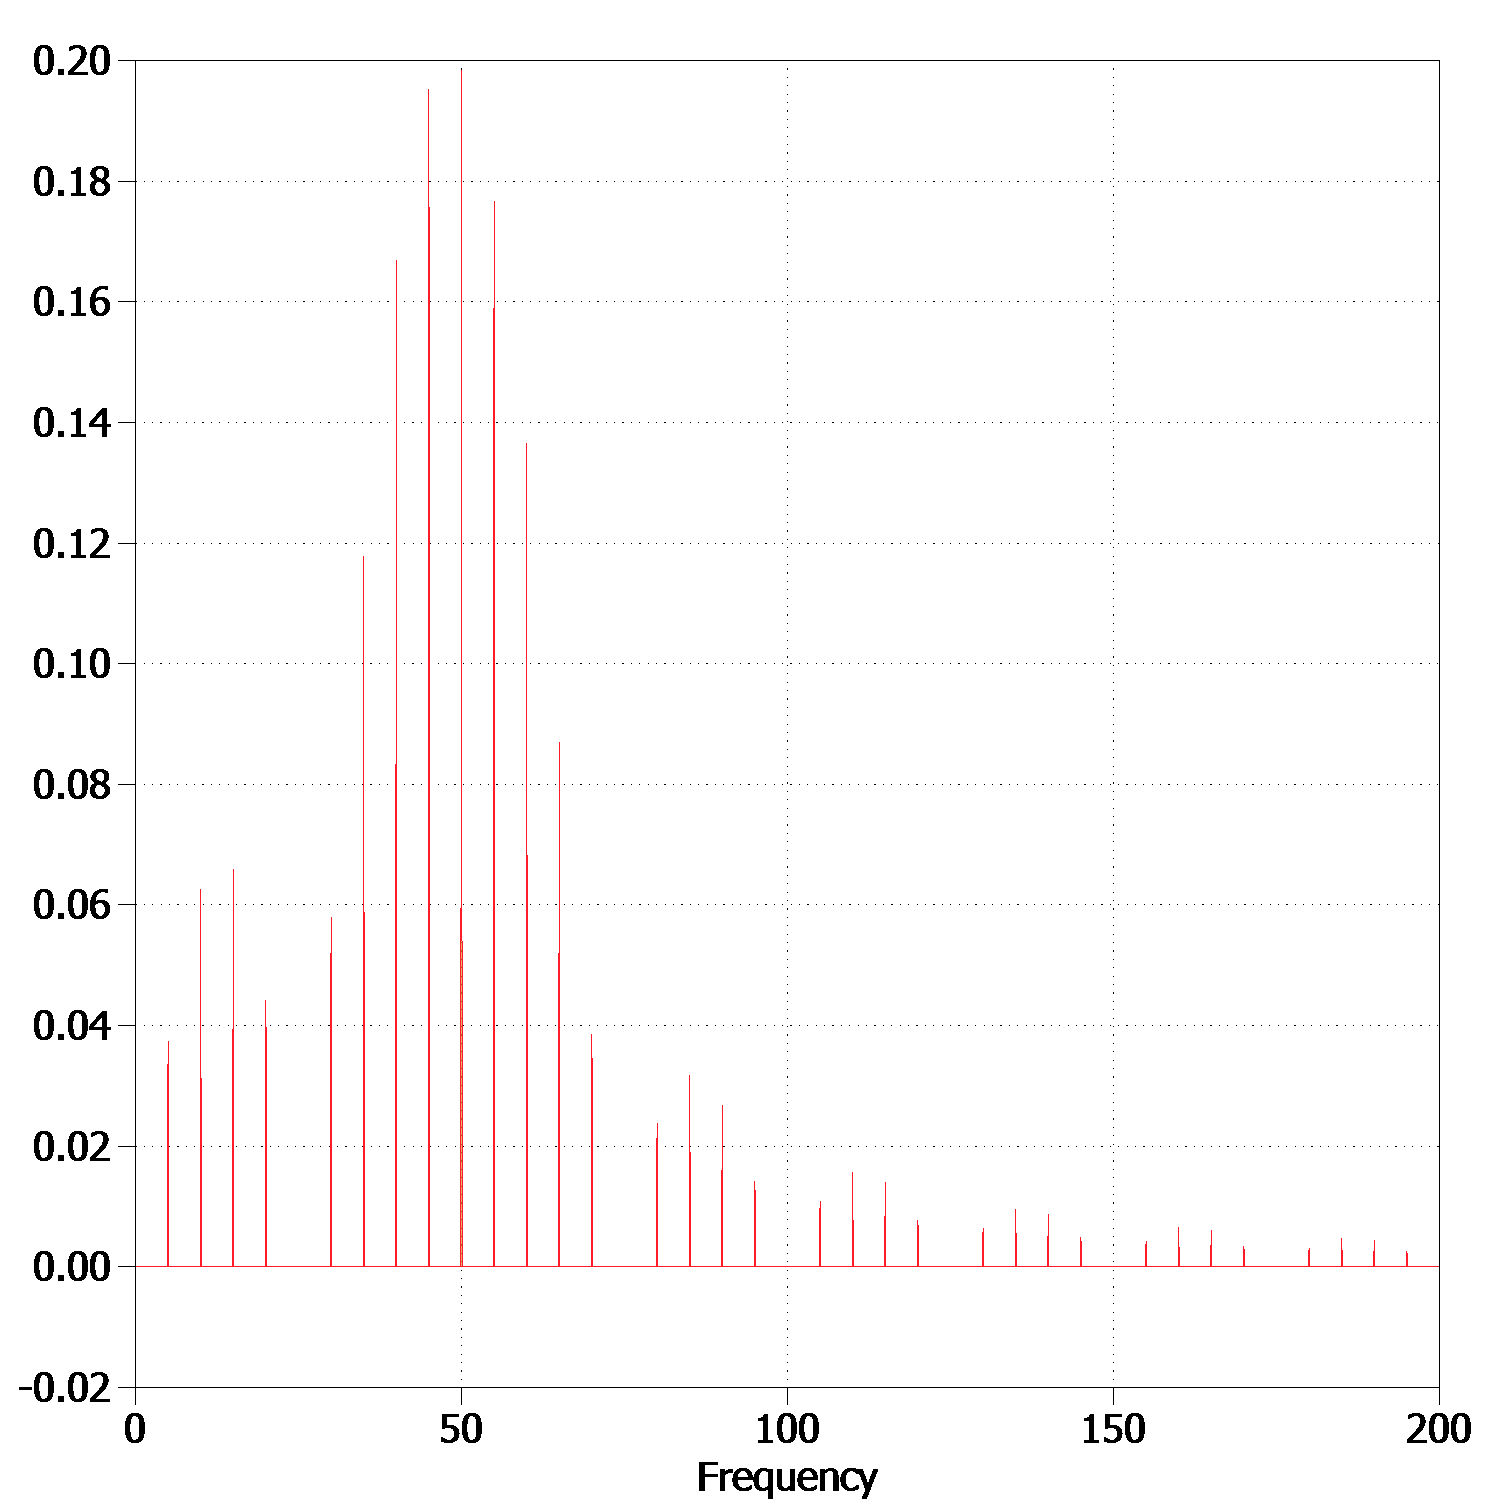
\includegraphics[scale=0.5]{sub_und_zwischenharmonische.png}	
	\caption{Sub- und Zwischenharmonische mit einer Grundfrequenz von 50 Hz}
	\label{fig:Sub und Zwischenharmonische}
\end{figure}

\newpage
\subsection{Phasenanschnittsteuerung}
Bei der Phasenanschnittsteuerung wird das Sinussignal über einen TRIAC geführt. Ein TRIAC sind zwei antiparallel geführt Thyristoren. Dieser zündet ab einem gewissen Zündwinkel nach jedem Nulldurchgang. Je später der TRIAC eingeschaltet wird, desto kleiner wird die mittlere Leistung über der Last. Ein Vorteil gegenüber einem Spannungsteiler ist, dass weniger Leistung gebraucht wird. Der Zündwinkel kann von 0\textdegree \hspace{0.02cm} bis 180\textdegree \hspace{0.02cm} eingestellt werden, wobei bei 0\textdegree \hspace{0.02cm} die maximale Leistung und bei 180\textdegree \hspace{0.02cm} keine Leistung über der Last anliegt. Das Problem bei der Phasenanschnittsteuerung ist, dass diese Schaltung Oberwellen produziert und so unerwünschte Effekte für den Netzbetreiber verursacht. Ein weiteres Problem betrifft den nicht-sinusförmigen Stromverlauf. Da Strom und Spannung nicht den gleichen Verlauf haben, tritt eine Verzerrungsblindleistung auf. Der Strom verläuft zeitlich der Spannung nach und wirkt so wie eine Induktivität. Deshalb wird dieses Verfahren von den Elektrizitätswerk nur bei kleinen Leistungen bis zu 200 Watt, bei symmetrischen Anschnittsteuerung von Wärmegeräten toleriert. Bei grösseren Leistungen wird deshalb die Schwinungspaketsteuerung verwendet. Auf der Abbildung \ref{fig:Phasenanschnitt1} ist ersichtlich, wie der Phasenanschnitt bei einer Netzspannung aussieht. Die Grau gezeichnete Kurve ist die normale Netzspannung und die rote ist die Spannung, welcher an der Last anliegt. In dieser Abbildung wurde ein Winkel von 135\textdegree \hspace{0.02cm} eingestellt. Die Leistung an der Last ist somit kleiner, als wenn die normale graue Netzspannung anliegen würde. 

\begin{figure}[ht!]
	\centering
	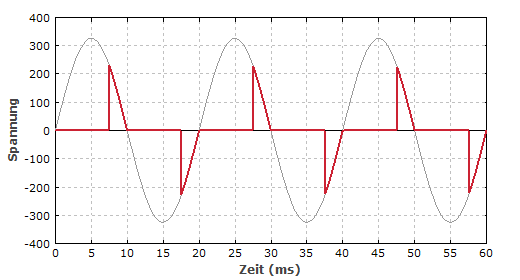
\includegraphics[scale=0.75]{phasenanschnittsteuerung1.png}	
	\caption{Phasenanschnitt mit einem Winkel von 135\textdegree \cite{Phasenanschnittsteuerung}}\label{fig:Phasenanschnitt1}
\end{figure}
\newpage
\begin{figure}[ht!]
	\centering
	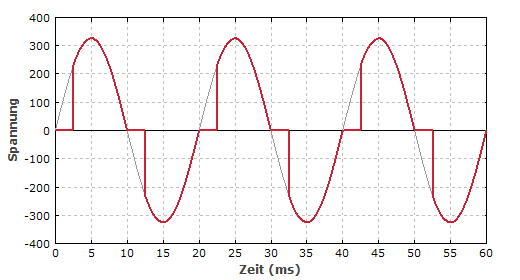
\includegraphics[scale=0.75]{phasenanschnittsteuerung2.png}	
	\caption{Phasenanschnitt mit einem Winkel von 45\textdegree \cite{Phasenanschnittsteuerung}}\label{fig:Phasenanschnitt2}
\end{figure}

In der Abbildung \ref{fig:Phasenanschnitt2} ist ersichtlich, dass die Phase früher gezündet wurde. Somit erhält man eine an der Last eine grössere Leistung.


\newpage
\subsection{Schwingungspaketsteuerung}
In diesem Verfahren wird nicht wie bei der Phasenanschnittsteuerung die Form der Halbwellen verändert, sondern die Zeitdauer der Halbwellen, welche an der Last anliegen. Wichtig sind dabei die Paketdauer $T_0$ und die Einschaltzeit $T_E$, wobei letzteres verändert wird. Wenn z.B. eine Paketdauer 10 Halbwellen hat, und 5 Halbwellen eingeschaltet sind, liegt die halbe Leistung über der Last an. Anders als bei der Phasenanschnittsteuerung enstehen bei dieser Ansteuerungsart keine harmonische Oberwellen, dafür aber Sub- und Zwischenharmonische. Auf der Abbildung \ref{fig:Schwingungspaketsteuerung} ist ersichtlich, wie vier von den total sechs Halbwellen pro Paket eingeschaltet sind. Dies ergibt eine Leistung welche ${2}/{3}$ so gross ist, wie die der normalen Netzspannung.

\begin{figure}[ht!]
	\centering
	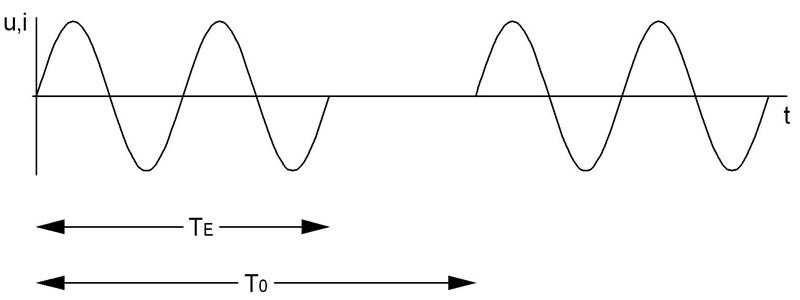
\includegraphics[scale=0.5]{Schwingungspaketsteuerung.png}	
	\caption{Schwingungspaketsteuerung ${2}/{3}$ der Leistung \cite{Schwingungspaketsteuerung}}\label{fig:Schwingungspaketsteuerung}
\end{figure}

Dabei ergibt sich aus dem Verhältnis von Einschaltdauer zu Periodendauer das Tastverhältnis.

\begin{equation}\label{eq:Einschaltverhältnis}
a = \frac{T_E}{T_0}
\end{equation}


%\subsection{TRIAC}
%Der TRIAC beseht aus zwei anti-parallele Thyristoren und kann über das Gate gezündet werden. Der TRIAC bleibt solange leitend bis der Haltestrom unterschritten wird. 

%\begin{figure}[ht!]
%	\centering
%	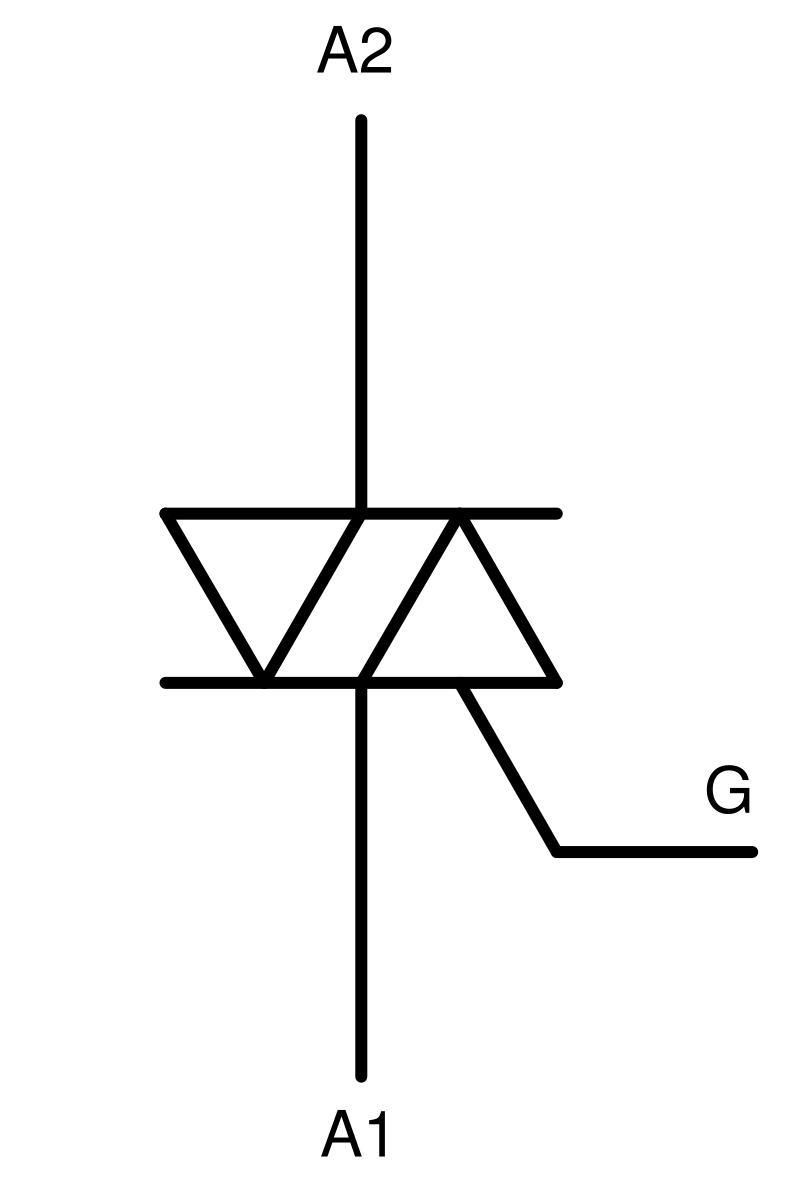
\includegraphics[scale=0.1]{TRIAC.png}	
%	\caption{Schaltzeichen eines TRIACs \cite{TRIAC}}\label{fig:TRIAC}
%\end{figure}


\subsection{Leistungsfaktor}
Um die zwei Ansteuerungsverfahren miteinander vergleichen zu können, wird der Leistungsfaktor benötigt. Bei der Phasenanschnittsteuerung ist der Leistungsfaktor abhängig von Zündwinkel. Bei der Schwingungspaketsteuerung ist der Leistungsfaktor abhängig vom Einschaltverhältniss. Die genaueren Berechnungen der Faktoren wird in der Formel \ref{eq:lamda_p_n} \& \ref{eq:lamda_s_n} beschrieben. 

In der Abbildung \ref{fig:Leistungsfaktor} ist ersichtlich wie der Leistungsfaktor bei den beiden Steuerungsarten aussieht. Bei der Phasenanschnittsteuerung auf der linken Seite sieht man, wie bei einem kleinem Zündwinkel der Leistungsfaktor sehr gross ist. Je grösser der Zündwinkel gewählt wird, desto kleiner wird der Leistungsfaktor. Auf der rechten Seite sieht man den Leistungsfaktor in Abhängigkeit des Einschaltverhältnisses. Je grösser das Einschaltzeitverhältnis, desto grösser der Leistungsfaktor \cite{Leistungselektronik}.
\begin{figure}[ht!]
	\centering
	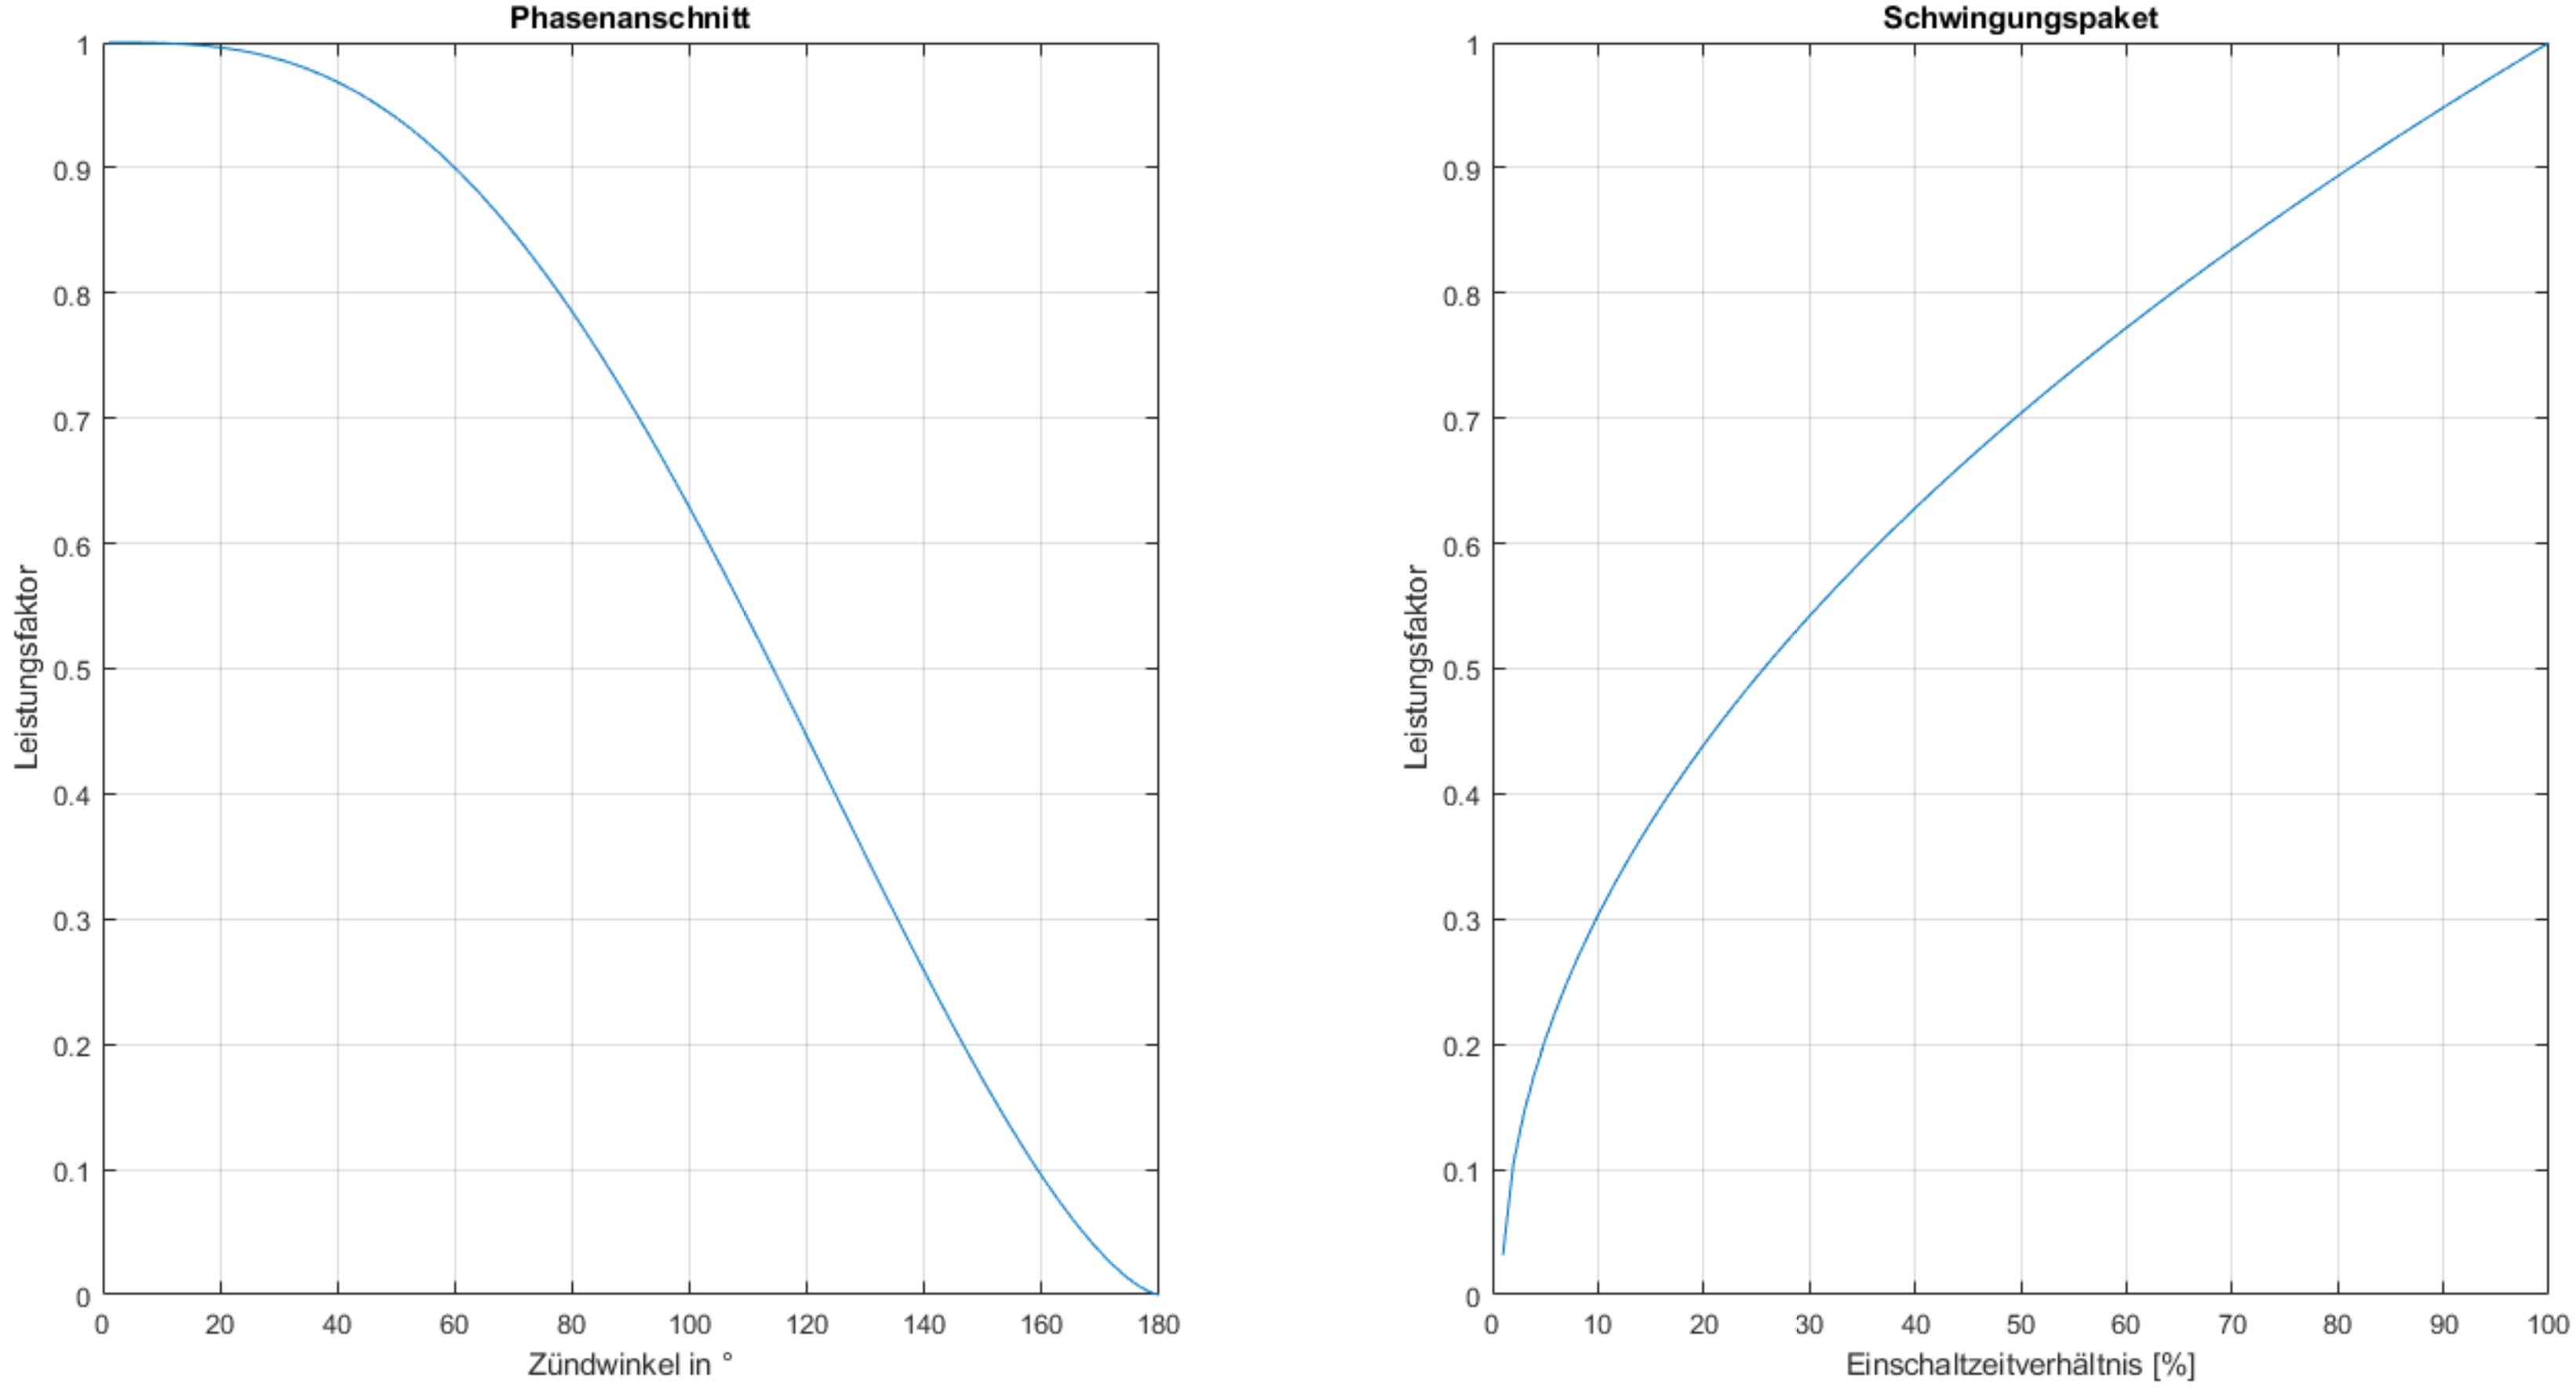
\includegraphics[width=\textwidth]{Leistungsfaktor.png}	
	\caption{Leistungsfaktor von Phasenanschnitt- und Schwingungspaketsteuerung}\label{fig:Leistungsfaktor}
\end{figure}
\newpage
\subsubsection{Leistungsfaktor Phasenanschnittsteuerung}
Der Leistungsfaktor ist definiert als Verhältnis von Wirkleistung zu Scheinleistung \cite{Leistungselektronik}. 
\begin{equation}\label{eq:lamda_p}
\lambda = \frac{P_{\alpha}}{S}
\end{equation}
Die Schein- und Wirkleistung können mit den folgenden Formeln beschrieben werden:
\begin{equation}\label{eq:Schein-&Wirkleistung}
\begin{array}{cc} 
S = I_L \cdot U_{UN}   &   P_{\alpha} = I_L^2 \cdot R_L  \\
\end{array}
\end{equation}
Werden die Formeln \ref{eq:Schein-&Wirkleistung} in die Formel \ref{eq:lamda_p} eingesetzt ergibt sich folgende Gleichung:
\begin{equation} \label{eq:Phas_1}
\frac{P_{\alpha}}{S} = \frac{I_L \cdot R_L}{U_{UN}}
\end{equation}
Der Laststrom wird mit folgender Formel beschrieben:
\begin{equation}
I_L = \sqrt{1-\frac{\alpha}{\pi}+\frac{1}{2\pi} \cdot sin(2\alpha)} \cdot \frac{U_{UN}}{R_L}
\end{equation}
Wenn die Formel für den Laststrom in die Gleichung \ref{eq:Phas_1} eingesetzt wird, lassen sich die Spannung und der Widerstand wegkürzen und übrig bleibt folgende Formel:
\begin{equation}\label{eq:lamda_p_n}
\lambda = \sqrt{1-\frac{\alpha}{\pi}+\frac{1}{2\pi} \cdot sin(2\alpha)}
\end{equation}

\newpage
\subsubsection{Leistungsfaktor Schwingungspaketsteuerung}
Das Einschaltsverhältnis wird als $a$ definiert und wird mit der Formel \ref{eq:Einschaltverhältnis} beschrieben.
Die Schein- und Wirkleistung haben das folgendem Verhältnis zum Einschaltverhältnis: \cite{Leistungselektronik}
\begin{equation}\label{eq:Schw_Schein-&Wirkleistung}
\begin{array}{cc} 
S_a = \sqrt{a} \cdot P  &   P_a = a \cdot P \\
\end{array}
\end{equation} 
Wenn die beiden Formeln für die Wirk- und Scheinleistung in die Gleichung für den Leistungsfaktor eingesetzt werden ergibt sich daraus folgende Gleichung: 
\begin{equation}
\lambda = \frac{P_a }{S_a} = \frac{a \cdot P}{\sqrt{a} \cdot P}
\end{equation}
Die Wirkleistung lässt sich wegkürzen und so ergibt sich folgende Formel:
\begin{equation}\label{eq:lamda_s_n}
\lambda = \sqrt{a}
\end{equation}

\todo{Einfügen was damit gemacht werden kann}

\subsection{Anforderung an die Netzqualität}

Um die Anforderungen der Netzqualität zu gewährleisten müssen die Normen eingehalten werden. Auf welche Nomen bei dieser Arbeit genau geachtete wurde, wird zu einem späteren Zeitpunkt erläutert. Zweck der Normen sind es  die verschiedene Merkmale wie zum Beispiel Frequenz, Höhe, Kurvenform oder die Symmetrie der drei Leiterspannungen einzuhalten. Durch Lastspannung, Störeinflüsse von bestimmten Anlagen oder Auftreten von Fehlern können diese Merkmale während des Normalbetriebes des Netzes geändert werden. 


\subsection{Gegenmassnahmen bei Oberschwingungen}

Es kann durchaus vorkommen, dass in der Praxis harmonische Oberschwingungen festgestellt wurden, welche die zulässigen Grenzwerte überschreiten. Es gibt jedoch Möglichkeiten diese zu verhindern und so die Netzqualität zu verbessern. Im folgenden Abschnitt werden auf ein paar Varianten eingegangen.

\subsubsection{Vermeidung von Störungen}
Das Vermeiden von Störungen ist die einfachste Art um eine Verbesserung der Netzqualität sicher zu stellen. Der Gesetzgeber liefert dafür Normen der Elektromagnetischen Verträglichkeit, welche den gesetzlichen Grundlagen entsprechen. Sie sind zwingend einzuhalten.
\subsubsection{Stromnetzeigenschaften}
Könnte man die Netzimpedanz verringern wäre eine Reduktion der Oberschwingungen möglich. Dies ist jedoch generell nicht umsetzbar und somit kann man Kurzschlussleistung des Netzes nicht beliebig erhöhen. Die wirtschaftlichen und technischen Grenzen sind hierzu massgebend.  


\subsubsection{Oberschwingungsfilter}

Zur Begrenzung von Oberschwingungen werden heutzutage  meistens mehrere aufeinander abgestimmte passive Filter eingesetzt. Das einsetzten von den Filtern muss jedoch für jede konkrete Installation neu erstellt werden, um eine Verbesserung des Netzrückwirkungsverhaltens zu erhalten.\\
Die Industrie entwickelte wegen diesem Problem aktive Oberschwingungsfilter. Sie können sich, auch bei späteren Erweiterungen der Installation, an die neu Situation anpassen und müssen nicht ersetzt werden. Ein weiterer Vorteil dieser Flexibilität des Filters ist es, dass die Nenngrösse einfach vom aktuellen Bedarf gewählt werden kann.     

\subsubsection{Änderung der Energieversorgung}

Stark nichtlineare Betriebsmittel und empfindliche Verbraucher die zusammen an einer Gruppe angeschlossen sind, können aufgetrennt und an separate Gruppen über jeweils einen separaten Transformator eingespeist werden. Eine solche Änderung der Energieversorgung sollte aber auch immer unter wirtschaftlichen Gesichtspunkten betrachtet werden.

\subsubsection{EMV verträgliche Gebäudeinstallation}

Um Schäden durch Oberschwingungen zu vermeiden müssen bei Gebäuden die Installation EMV-verträglich sein.
Folgende Punkte sollten dabei zwingend beachtet werden:

\begin{itemize}
	\item Es sollte ein konsequentes TN-S-Netz mit getrenntem Neutral- und Schutzleiter aufgebaut werden. Die beiden Leiter sollten nur eine Verbindung zwischen einem Punkt haben.
	\item Um Schäden an einer Anlage zu vermeiden wäre ein Überspannungsschutz für Kompensationsanlagen von Vorteil.
	\item Wie schon erwähnt, wären getrennte Stromkreisgruppen für allgemeine und IT-Betriebs-mittel vorteilhaft.
	\item Leitende oder metallene Teile, wie zum Beispiel Trasse, Rohre oder Lüftungskanäle sollten zwingend mit dem Potentialausgleich verbunden werden.
	
\end{itemize}

Auch die Energieversorgung bei der Gebäudeinstallation sollte EMV-verträglich sein. Folgende Punkte sollten dabei eingehalten werden. 

\begin{itemize}
	\item Das Erdungssystem sollte niederohmig und stromfähig installiert sein.
	\item Im Schutzleiter- und Potenzialausgleich-Systeme sollten keine Arbeitsströme zugelassen sein.
	\item Bei Mehrfacheinspeisung dürfen keine Mehrfacherdung des Neutralleiters zugelassen werden.
	\item Der Kabelquerschnitt sollte für die Oberschwingungen ausgelasstet sein.
\end{itemize}  






\subsection{Normen}
Bei der Formulierung "Normen" handelt es sich um eine Herausgabe von Regeln, Merkmale oder Leitlinien, die von verschiedenen Organisatoren und deren Expertengruppen bestimmt wurden. Die gesicherten Ergebnisse, welche auf Wissenschaft, Technik und Erfahrung basieren, dokumentierte man sorgfältig zum Beispiel in den EN-Normen. Sie sollen einen optionalen Vorteil für die Gesellschaft und eine bestimmte Qualität erhalten.\\
Im folgenden Unterkapitel gibt es eine kurze Zusammenfassung der Normen, die für diese Arbeit als wichtig empfunden wurde. Es handelt sich dabei vor allem um die Spannungsqualität, welche man aus verschiedene Blickwinkeln angeschaut hat. Die Normen EN 61000-3-2 und EN 61000-3-3 (Grenzwerte für Oberschwingungsströme, Spannungsänderungen, Spannungsschwankungen und Flicker im öffentlichen Netz) beschreiben, welche Spannungsänderung ein Elektrogerät haben darf, damit die ins öffentliche Stromnetz hinein übertragenen Störungen in Grenzen gehalten werden. Eine weitere Norm, welche betrachtet wurde, ist die EN 61000-2-2. Bei dieser Norm handelt es sich um die elektromagnetische Verträglichkeit bei Umgebungsbedingungen für niederfrequente, leitungsgeführte Störgrössen und Signalübertragung in die öffentlichen Versorgungsnetze.\\
Die betrachteten Normen sind in diesem Bericht nicht im Detail erläutert. Nur die für uns wichtigen Teile sind zusammengefasst. Für weitere Segmente können die Normen nachgelesen werden. 


\subsubsection{EN 61000-3-2}
Diese Norm gilt für elektrische und elektronische Geräte (Betriebsmittel und Einrichtungen) bis zu einem Eingangsstrom von \SI{16}{HZ} je Leiter. Ausserdem ist der Anschluss des Gerätes an das öffentliche Niederspannungs-Verteilnetz vorgesehen. Unter dem Begriff Elektrische Einrichtung versteht man eine Anlage, welches aus einem oder mehreren voneinander unabhängigen Geräten besteht. Sie bilden dann eine elektrische Einrichtung, wenn nur durch deren Zusammenwirken der bestimmungsgenässe Zweck der Einrichtung erzielt werden kann. Ein Beispiel wäre, bei einer elektrischen Einrichtung, der Treppenlichtautomat zusammen mit den dazugehörigen Leuchten. Nur der Automat ohne Beleuchtung erfüllt den technischen Zweck nicht. Ein weiteres Beispiel für eine Elektrische Einrichtung wäre der motorische Antrieb. Aber auch hier gilt, dass der Motor ohne mechanische Last den technischen Nutzen nicht erfüllen würde. Bei einem elektrischen Gerät handelt es sich zum Beispiel um einen Backofen und die dazu gehörigen einzelne Kochmodule eines Multifunktions-Herdes.\\
Die Norm definiert die Grenzwerte der Oberschwingungsanteile des Eingangsstromes bis zur 40 Harmonischen, die durch ein Gerät hervorgerufen werden können, das unter festgelegten Bedingungen geprüft wird. Da heutzutage die Zahl der nicht linearen Verbraucher am öffentlichen Versorgungsnetz zunehmend steigen, steigt auch der Anteil des Oberschwingungsgehalts der Versorgungsspannung. Schaltnetzteile, Audio-Verstärker, Beleuchtungseinrichtungen aber auch Waschmaschinen, Mikrowellenöfen oder Klimageräte sind typische Verursacher von solchen Oberschwingungen.
Die nicht-sinusförmige und somit oberschwingungsbehaftete Stromentnahme verursacht an der Netzimpedanz Spannungsabfälle. Das Resultat ist eine Abweichung des Spannungsverlaufs von dem idealen harmonischen Verlauf des Netzes. Um normgerechte und reproduzierbare Messungen der Stromoberschwingungen durchführen zu können, muss ein ideales oberschwingungsfreies Netz zur Verfügung stehen. Laut der Norm EN 61000-3-2 darf die Prüfquelle eine bestimmten Oberwellengehalt nicht überschreiten. Es muss sichergestellt werden, dass ausschliesslich die vom Verbraucher erzeugte Stromoberschwingung gemessen werden. Beginnt man mit der Prüfung, muss der Prüfling so eingestellt werden, dass der höchste Gesamt-Oberschwingungsstrom (maximal total harmonic current) unter üblichen Betriebsbedingungen erreicht wird.
Für die Quellenanforderung gelten folgende Spezifikationen, die zwingend, während des zu prüfenden Geräts, eingehalten werden müssen:

\begin{itemize}
\item Spannungsgenauigkeit $\pm$ 2 \%
\item Frequenzgenauigkeit $\pm$ 0.5 \%
\item Phasenwinkelstabilität $\pm$ $1.5^\circ$
\item 	U$_{peak}$ = \SI{1.4}{V} - \SI{1.42}{V} U$_{eff}$ und zwischen 87\textdegree \hspace{0.02cm} und 93\textdegree \hspace{0.02cm} nach dem Nulldurchgang erreicht werden, dies muss jedoch nicht eingehalten werden, sofern Klasse A oder B geprüft wird.
\item Die relativen Oberschwingungsanteile der Prüfspannung dürfen folgende Werte nicht überschreiten
0.9 \% für die 3. Harmonische Oberschwingung\\
0.4 \% für die 5. Harmonische Oberschwingung\\
0.3 \% für die 7. Harmonische Oberschwingung\\
0.2 \% für die 9. Harmonische Oberschwingung\\
0.2 \% für die geradzahlige Oberschwingung 2 bis 10 Ordnung\\
0.1 \% für die Oberschwingung 11 bis 40 Ordnung\\
\end{itemize} 

In der Norm 61000-3-2 sind 4 Geräteklassen definiert, bei denen die Oberschwingungen des Eingangsstromes die Werte nicht überschreiten dürfen. Da es sich bei dem Projekt um symmetrische, dreiphasige ohmsche Lasten handelt, fällt dies unter die Klasse A. Ausserdem beinhalten die folgenden Einrichtungen auch die Klasse A. 
\begin{itemize}
\item Symmetrische dreiphasige Geräte	
\item Haushaltsgeräte (ausser die, die in Klasse D fallen)
\item Elektrowerkzeuge (ausser tragbare Elektrowerkzeuge)
\item Beleuchtungsregler (Dimmer) für Glühlampen
\item Audio-Einrichtungen
\end{itemize} 

Um zu verdeutlichen, welche Geräte die anderen Klasse erhalten, sind sie Vollständigkeit halber auch noch aufgelistet.\\
Klasse B:
\begin{itemize}
	\item tragbare Elektrowerkzeuge 	
	\item Lichtbogenschweisseinrichtungen, die nicht zum professionellen Gebrauch vorgesehen sind.
\end{itemize} 
Klasse C:
\begin{itemize}
	\item Beleuchtungseinrichtungen	
\end{itemize} 
Klasse D:
\begin{itemize}
	\item Personalcomputer und Bildschirme (Monitore) für Personalcomputer	
	\item Fernseh-Rundfunkempfänger
\end{itemize}

\newpage
Falls es Geräte gibt, die nicht in die Klassen B bis D fallen, müssen sie automatisch als Geräte der Klasse A definiert werden.\\
Die Grenzwerte für den Höchstwert des Oberschwingungsstromes für Klasse A Geräte sind wie folgt definiert:

\begin{table}[ht!]
	\centering
	\begin{tabular}{|l|l|}
		\hline
		\multicolumn{1}{|c|}{Oberschwingungsordnung} & \multicolumn{1}{c|}{\begin{tabular}[c]{@{}c@{}}Zuverlässiger Höchstwert des \\ Oberschwingungsstromes\end{tabular}} \\
		\multicolumn{1}{|c|}{\textit{n}}                      & \multicolumn{1}{c|}{A}                                                                                              \\ \hline
		\multicolumn{2}{|c|}{Ungeradzahlige Oberschwingungen}                                                                                                              \\ \hline
		3                                            & 2.30                                                                                                                \\
		5                                            & 1.14                                                                                                                \\
		7                                            & 0.77                                                                                                                \\
		9                                            & 0.40                                                                                                                \\
		11                                           & 0.33                                                                                                                \\
		13                                           & 0.21                                                                                                                \\
		15 $\leq$ \textit{n} $\leq$ 39               & 0.15 x 15/\textit{n}                                                                                                \\ \hline
		\multicolumn{2}{|c|}{Geradzahlige Oberschwingungen}                                                                                                                \\ \hline
		2                                            & 1.08                                                                                                                \\
		4                                            & 0.43                                                                                                                \\
		6                                            & 0.30                                                                                                                \\
		8 $\leq$ \textit{n} $\leq$ 40                & 0.23 x 8/\textit{n}                                                                                                 \\ \hline
	\end{tabular}
\caption{Grenzwerte für Geräte der Klasse A}\label{Test}
\end{table}


Ein weiterer wichtiger Wert, ist die jeweilige Beobachtungsdauer der Endgeräte. Es wurden 4 verschiedene Arten von Geräteverhalten definiert und dabei die Beobachtungsdauer bestimmt. Dies sieht man in der folgenden Tabelle:

\begin{table}[ht!]
	\centering
	\begin{tabular}{|l|l|}
		\hline
		\multicolumn{1}{|c|}{Art des Geräteveraltens}                      & \multicolumn{1}{c|}{Beobachtungsdauer}                                                                                                                                                                                   \\ \hline
		quasi-stationär                                                    & \begin{tabular}[c]{@{}l@{}}T$_{obs}$ von ausreichender Dauer, um die Anforderungen\\ zur Wiederholpräzision einzuhalten\end{tabular}                                                                                          \\ \hline
		kurzer Zyklus (T$_{cycle}$ $\leq$ 2.5min)                                    & \begin{tabular}[c]{@{}l@{}}T$_{obs}$ $\geq$ 10 Zyklen (Bezugsverfahren) oder T$_{obs}$ von \\ ausreichender Dauer oder Synochronisation, um \\ die Anforderungen zur Wiederholpräzision\\ einzuhalten \hspace{0.1cm}$^a$\end{tabular}                      \\ \hline
		zufällig                                                           & \begin{tabular}[c]{@{}l@{}}T$_{obs}$ von ausreichender Dauer, um die Anforderungen\\ zur Wiederholpräzision einzuhalten\end{tabular}                                                                                          \\ \hline
		langer Zyklus (T$_{cycle}$ \textgreater 2.5 min)                        & \begin{tabular}[c]{@{}l@{}}voller Programmzyklus des Gerätes (Bezugsverfahren)\\ oder ein repräsentives 2.5 min -Intervall mit dem \\ höchsten THC angesehen wird\end{tabular}                                           \\ \hline
		\multicolumn{2}{|l|}{\begin{tabular}[c]{@{}l@{}} $^a$ \grqq Synchronisation\grqq \hspace{0.08cm} bedeutet, dass die gesamte Beobachtungsdauer hinreichend gut eine\\ exakte ganzzahlige Anzahl von Betriebszyklen des Gerätes umfasst, so dass die\\Anforderungen zur Wiederholpräzision eingehalten wird.\end{tabular}} \\ \hline
	\end{tabular}
	\caption{Beobachtungsdauer für die Prüfung}\label{Test2}
\end{table}

Am Ende der Prüfung muss ein Prüfbericht abgegeben werden, der alle relevanten Informationen zu den Prüfbedingungen, die Beobachtungsdauer der Prüfung sowie die Wirkleistung oder den Grundschwingungsstrom und den Leistungsfaktor beinhalten. Dies gilt auch bei den anderen Normen.

\subsubsection{EN 61000-3-3}
Auch diese Norm gilt für Geräte und Einrichtungen mit einem Nenn-Eingansstrom von bis zu \SI{16}{A} je Aussenleiter, die zum Anschluss an das öffentliche Niederspannungsnetz vorgesehen sind und keiner Sonderanschlussbedingung unterlegen. Die Flicker, die auch als repetitive Spannungsänderungen bekannt sind, die Spannungsschwankungen und die allgemeinen Spannungsänderungen, können so begrenzt werden. Falls Geräte und Einrichtungen diese Norm erfüllen, dürfen sie ohne weitere Prüfung an jeden Anschlusspunkt des öffentlichen Netzes angeschlossen werden. Die Nennleistung, welche die Geräte und Einrichtungen aufweisen sollten, sind ohne Einschränkungen kleiner als \SI{11}{kW} bei Drehstromgeräten, \SI{3.7}{kW} bei Einphasengeräten und \SI{6.47}{kW} bei Zweiphasengeräten. Diese Norm trifft man unter anderem beifolgenden Geräten an:
\begin{itemize}
\item Haushaltsgeräte und tragbare Elektrowerkzeuge 
\item Motorbetriebene Geräte (Waschmaschine, Staubsauger, Elektrowärmegerät und Kocheinrichtungen)
\item Beleuchtungseinrichtungen
\item Automatische elektrische Steuerungen für Hausgebrauch und ähnliche Anwendungen
\item Drehzahlgeregelte Antriebe
\item Funk-Einrichtungen
\item Lichtbogenschweisseinrichtungen
\item Medizinische Geräte und Einrichtungen
\item Mikrowellengeräte	
\end{itemize}

Die Norm schreibt eine Prüfung, der zu beurteilenden Geräten, an einer Prüfungsimpedanz vor. Die Impedanz $Z$ ist im unteren Bild als Widerstand R$_A$ in Serie mit einer Spule jX$_A$ dargestellt und entspricht den folgenden Werten:


\begin{figure}[ht!]
	\centering
	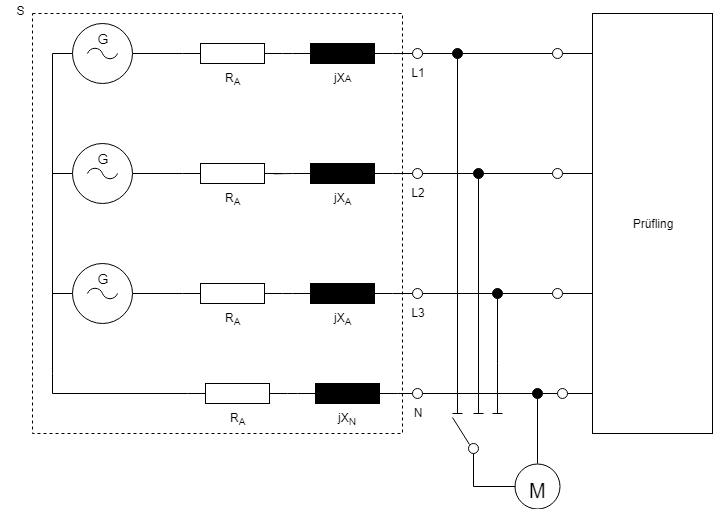
\includegraphics[scale=0.4]{Bezugsimpedanz.png}	
	\caption{Prüfspannungsquelle mit der Bezugsimpedanz}
	\label{fig:Bezugsimpedanz}
\end{figure}

\begin{table}[ht!]
	\begin{tabular}{ll}
		G  & Spannungsquelle                                                                                                                                                                                                                                               \\
		M  & Messeinrichtung                                                                                                                                                                                                                                               \\
		S  & \begin{tabular}[c]{@{}l@{}}Prüfungspannungsquelle, bestehend aus dem Spannungsgenerator  G und der\\ Bezugsimpedanz Z mit den Elemente\end{tabular}                                                                                                           \\
		& \begin{tabular}[c]{@{}l@{}}R$_A$ = $\SI{0.24}{\Omega}$  jX$_A$ = $\SI{0.15}{\Omega}$ bei $\SI{50}{Hz}$\\ R$_N$ = $\SI{0.16}{\Omega}$ jX$_A$ = $\SI{0.10}{\Omega}$ bei $\SI{50}{Hz}$\end{tabular}
	\end{tabular}
\end{table}

Die drei Quellenspannungen $G$ entsprechen der Nennspannung. Alle Spannungen werden auf die Nennspannung $Un$ normiert: Der Prüfkreis besteht aus der Prüfspannungsquelle, dem zu prüfenden Gerät (Prüfling) und einer Messeinrichtung z.B. Strommesser, Spannungszange oder einem Flickermeter (M).\\


Es gibt bei der Bezugsimpedanz keine Unterscheidung im Anwendungsbereich zwischen Haushaltsgeräten und gewerblich genutzten Geräten. Stattdessen wird die Langzeit-Flickerstärke eingeführt und auf 65 \% der Kurzzeit-Flickerstärke begrenzt.\\
Mit Hilfe des Flickerwertes kann man die Störempfindlichkeit des menschlichen Auges, auf Helligkeitsschwankungen bei der Beleuchtung, durch einen messbaren Wert ermitteln. Dieser Wert ist eine dimensionslose Zahl, welche das Störempfinden des Menschen ausdrückt, wenn er sich mit einer \SI{60}{W} Glühbirne beleuchtet. Die Helligkeit variiert dabei auf Grund von Spannungsschwankungen.
Erhält man den Wert 0 so bedeutet dies, dass praktisch keine Schwankungen der Spannungshöhe vorhanden und somit auch kein Flackern der Lampe ersichtlich ist.\\
Bei dem Wert 1 gibt es eine gewisse Helligkeitsschwankung, die als störend wahrgenommen wird. Jedoch sind die Resultate nicht aussagekräftig, da sie Orts-, Zeit- und Personen abhängig sind. Deshalb entwickelte man einen Algorithmus und ein entsprechendes Formelwerk für das Durchschnittsempfinden der Erkenntnisse. Mit Hilfe eines Flicker-Meter konnte ein geeignets Messgerät entwickelt werden, welches mit einem Flickermessverfahren den Flickerwert berechnen konnte. Das Flicker-Meter liefert alle 10 Minuten einen Wert, der mit $Pst$ bezeichnet wird. Das $P$ steht dabei für $perceptibility units$ (Wahrnehmungseinheiten) und $st$ steht für $short time$. Der Wert, welcher man behandelt ist also der Kurzzeit-Flickerwert.\\
Die EN 50160 Norm sagt aus, dass man 12 aufeinander folgende $Pst-Werte$ zusammenfassend zu einem $Plt-Wert$ (long time-Flicker = Langzeit-Flicker) verrechnen kann. Genauer bedeutet dies, dass man die 12 $Pst-Werte$, die über 2 Stunden gemessen wurden, zusammenrechnet und daraus den Durchschnitt nimmt. Jeder einzelne $Pst-Wert$ geht mit einer 3. Potenz in die Bewertung ein. Der $Plt-Wert$ ist also der kubische Mittelwert der 12 $Pst-Werte$ und ist in der unterstehenden Formel dargestellt.


\begin{equation}\label{eq:THDi}
P_{lt} = {\sqrt[3]{\frac{\sum_{i=1}^{N} {P_{st,i}}^3}{N}}}
\end{equation}


Alle Spannungen werden auf die Nennspannung U\textsubscript{n} normiert:
relative Spannungsänderung:
\begin{equation}\label{eq:relative Spannungsänderung}
d = \frac{\Delta U}{ U_n}
\end{equation}
relative Spannungsänderungsverlauf
\begin{equation}\label{eq:relative Spannungsänderungsverlauf}
d(t) = \frac{\Delta U(t)}{ U_n}
\end{equation}
relative konstante Spannungsabweichung
\begin{equation}\label{eq:relative konstante Spannungsabweichung}
d_c = \frac{\Delta U_c}{ U_n}
\end{equation}
grösste relative Spannungsänderung
\begin{equation}\label{eq:grösste relative Spannungsänderung}
d_{max} = \frac{\Delta U_{max}}{ U_n}
\end{equation}
relative Spannungsschwankung
\begin{equation}\label{eq:relative Spannungsschwankung}
d(t) = \frac{\Delta U(t)}{ U_n}
\end{equation}


Mit Hilfe dieser Norm können Typenprüfung für bestimmte Geräte vorgenommen werden. Das Ziel dieser Typenprüfung ist es, die Übereinstimmung mit den Grenzwerten festzustellen. Diese werden unter Laborbedingungen an einem Bezugsnetz betrieben. Bei den festgelegten Betriebsbedingungen werden die erzeugten Spannungsschwankungen in Bezug auf die Bezugsimpedanzen gemessen und beurteilt. Falls Geräte die Grenzwerte dieser Norm einhalten, kann davon ausgegangen werden, dass sie zu keinerlei Beschwerden im Netz Anlass geben. Die elektromagnetische Verträglichkeit ist daher gewährleistet. 


\subsubsection{EN 61000-2-2}

Die folgende Norm beinhaltet die Festlegung für Verträglichkeitspegel von niederfrequenten, leitungsgeführten Störgrössen und für Signale von Netz-Kommunikationssystemen in öffentlichen Niederspannungs- und Stromversorgungsnetzen. Die Werte des Verträglichkeitspegels mit ihrer Eigenschaft können für die EMV-Koordinierung von Störaussendungs- und Störfestigkeitsanforderungen für Geräte und als Planungspegel für Stromversorgungsnetze verwendet werden. In der Norm werden folgende Phänomene betrachtet:

\begin{itemize}
	\item Spannungsschwankungen und Flicker 
	\item Oberschwingungen bis zur 50. Oberschwingungsordnung
	\item Zwischenharmonische
	\item Spannungsverzerrungen bei Frequenzen oberhalb der 50. Oberschwingungsordnung
	\item Spannungseinbrüche
	\item Kurzzeitunterbrechungen der Versorgungsspannung
	\item Spannungsunsymmetrien
	\item Kurzzeitunterbrechungen der Versorgungsspannung
	\item Transiente Überspannung
	\item Zweiteilige Schwankung der Netzfrequenz
\end{itemize}
Wobei man sagen kann, dass einige Punkt, wie zum Beispiel das bestimmen des Flickerwertes oder die langzeit- und die Kurzzeit Flickerstärke, schon in der vorherigen Norm definiert wurde.\\
Die folgende Tabelle zeigt die verschiedenen Kompatibilitätsstufen für einzelne Oberschwingungsspannungen im Niederspannungsnetz. Sie ist aber nur in Bezug auf Langzeiteffekte für einzelne harmonische Spannung definiert. Der Wert der gesamten harmonische Verzerrung darf hierbei höchstens einen Wert von THD = 8\% betragen.
\begin{table}[ht!]
	\centering
	\resizebox{\textwidth}{!}{%
		\begin{tabular}{|l|l|l|l|l|l|}
			\hline
			\multicolumn{2}{|c|}{\begin{tabular}[c]{@{}c@{}}Ungeradzahlige \\ Harmonische \\ nicht-vielfache von 3\end{tabular}}                                                            & \multicolumn{2}{c|}{\begin{tabular}[c]{@{}c@{}}Ungeradzahlige \\ Harmonische \\ Vielfache von 3\end{tabular}}                                                                     & \multicolumn{2}{c|}{\begin{tabular}[c]{@{}c@{}}Geradzahlige \\ Harmonische\end{tabular}}                                                                                          \\ \hline
			\multicolumn{1}{|c|}{\begin{tabular}[c]{@{}c@{}}Oberschwingungs\\ -ordnung\end{tabular}} & \multicolumn{1}{c|}{\begin{tabular}[c]{@{}c@{}}Harmonische \\ Spannung\end{tabular}} & \multicolumn{1}{c|}{\begin{tabular}[c]{@{}c@{}}Oberschwingungs\\ -ordnung\end{tabular}} & \multicolumn{1}{c|}{\begin{tabular}[c]{@{}c@{}}Harmonische \\ Spannung\end{tabular}} & \multicolumn{1}{c|}{\begin{tabular}[c]{@{}c@{}}Oberschwingungs\\ -ordnung\end{tabular}} & \multicolumn{1}{c|}{\begin{tabular}[c]{@{}c@{}}Harmonische \\ Spannung\end{tabular}} \\
			\multicolumn{1}{|c|}{\textit{h}}                                                                  & \multicolumn{1}{c|}{\%}                                                              & \multicolumn{1}{c|}{\textit{h}}                                                                     & \multicolumn{1}{c|}{\%}                                                              & \multicolumn{1}{c|}{\textit{h}}                                                                     & \multicolumn{1}{c|}{\%}                                                              \\ \hline
			5
			5                                                         & 6                                                     & 3                                                       & 5                                                & 2                                           & 2                                         \\
			7                                                         & 5                                                     & 9                                                       & 1.5                                              & 4                                           & 1                                         \\
			11                                                        & 3.5                                                   & 15                                                      & 0.4                                              & 6                                           & 0.5                                       \\
			13                                                        & 3                                                     & 21                                                      & 0.3                                              & 8                                           & 0.5                                       \\
			17 $\leq$\textit{h}$\leq$ 49                                                   & 2.27x(17/\textit{h})-0.27                                   & 21<h$\leq$45                                                 & 0.2                                              & 10$\leq$\textit{h}$\leq$50                                     & 0.25x(10/\textit{h})+0.25                       \\ \hline
	\end{tabular}}
	\caption{Kompatibilitätsstufen für einzelne Oberschwingungsspannungen im Niederspannungsnetz}\label{Test1}
\end{table}

Bei Kurzzeiteffekten wird ein Faktor k zu den harmonischen Ordnungen hinzu multipliziert. Dieser Faktor wird wie folgt berechnet: 
\begin{equation}\label{eq:factor_k_für_kurzzeiteffekte}
k = {1.3+\frac{0.7}{45}\cdot(h-5)}
\end{equation}
Der entsprechende Kompatibilitätsgrad für die gesamte harmonische Verzerrung liegt daher bei THD = 11\%.



Die unterstehende Tabelle zeigt die erforderlichen Werte in Prozent der subharmonischen Spannung im Niederspannungsnetz bei \SI{230}{V}, bei einer Frequenz von \SI{10}{Hz} bis \SI{90}{Hz}. Sie entsprechen dem Kompatibilitätsgrad bezüglich des Flimmerns.
\begin{table}[ht!]
	\centering
	\begin{tabular}{|l|l|l|}
		\hline
		\multicolumn{1}{|c|}{\multirow{3}{*}{\begin{tabular}[c]{@{}c@{}}Ordnung\\   {[}m{]}\end{tabular}}} & \multicolumn{2}{c|}{50 Hz System}                                                                                                                    \\ \cline{2-3} 
		\multicolumn{1}{|c|}{}                                                                             & \multicolumn{1}{c|}{\multirow{2}{*}{\begin{tabular}[c]{@{}c@{}}Subharmonische\\   Frequenzen fm {[}Hz{]}\end{tabular}}} & \multicolumn{1}{c|}{Um \%} \\ \cline{3-3} 
		\multicolumn{1}{|c|}{}                                                                             & \multicolumn{1}{c|}{}                                                                                                   & \multicolumn{1}{c|}{230V}  \\ \hline
		0.20 < m $\leq$ 0.60                                                                              & 10 < fm $\leq$ 30                                                                                                    & 0.51                        \\ \hline
		0.60 < m $\leq$ 0.64                                                                             & 30 < fm $\leq$ 32                                                                                                    & 0.43                        \\ \hline
		0.64 < m $\leq$ 0.68                                                                            & 32 < fm $\leq$ 34                                                                                                    & 0.35                        \\ \hline
		0.68 < m $\leq$ 0.72                                                                            & 34 < fm $\leq$ 36                                                                                                    & 0.28                        \\ \hline
		0.72 < m $\leq$ 0.76                                                                            & 36 < fm $\leq$ 38                                                                                                    & 0.23                        \\ \hline
		0.76 < m $\leq$ 0.84                                                                            & 38 < fm $\leq$ 42                                                                                                    & 0.18                        \\ \hline
		0.84 < m $\leq$ 0.88                                                                            & 42 < fm $\leq$ 44                                                                                                    & 0.18                        \\ \hline
		0.88 < m $\leq$ 0.92                                                                            & 44 < fm $\leq$ 46                                                                                                    & 0.24                        \\ \hline
		0.92 < m $\leq$ 0.96                                                                            & 46 < fm $\leq$ 48                                                                                                    & 0.36                        \\ \hline
		0.96 < m $\leq$ 1.04                                                                            & 48 < fm $\leq$ 52                                                                                                    & 0.64                        \\ \hline
		1.04 < m $\leq$ 1.08                                                                            & 52 < fm $\leq$ 54                                                                                                    & 0.36                        \\ \hline
		1.08 < m $\leq$ 1.12                                                                            & 54 < fm $\leq$ 56                                                                                                    & 0.24                        \\ \hline
		1.12 < m $\leq$ 1.16                                                                            & 56 < fm $\leq$ 58                                                                                                    & 0.18                        \\ \hline
		1.16 < m $\leq$ 1.24                                                                            & 58 < fm $\leq$ 62                                                                                                    & 0.18                        \\ \hline
		1.24 < m $\leq$ 1.28                                                                            & 62 < fm $\leq$ 64                                                                                                    & 0.23                        \\ \hline
		1.28 < m $\leq$ 1.32                                                                            & 64 < fm $\leq$ 66                                                                                                    & 0.28                        \\ \hline
		1.32 < m $\leq$ 1.36                                                                            & 66 < fm $\leq$ 68                                                                                                    & 0.35                        \\ \hline
		1.36 < m $\leq$ 1.40                                                                             & 68 < fm $\leq$ 70                                                                                                    & 0.43                        \\ \hline
		1.40 < m $\leq$ 1.80                                                                              & 70 < fm $\leq$ 90                                                                                                    & 0.51                        \\ \hline
	\end{tabular}
	\caption{}\label{Test3}
\end{table}

Einige Effekte, die wegen subharmonische Oberschwingung entstehen können sind:
\begin{itemize}
	\item Unerwünschter Strom, der in die Versorgungsnetze fliesst, welcher zusätzlicher Energieverlust verursacht.
	\item Subharmonische Spannungen stören den Betrieb von Leuchtstofflampen und anderen elektronischen Geräte, wie zum Beispiel Fernsehempfängern. Jede Verwendung von Strom und Spannungen, bei der die Höhe der Amplitude oder der Zeitpunkt des Nulldurchgangs wichtig ist, kann somit gestört werden, wenn die Kombination der vorhandenen unerwünschten Frequenz diese Eigenschaften der Versorgungsspannung ändern.
	\item Je grösser der Frequenzbereich ist und je grösser die Amplitude der Spannung bei diesen Frequenzen sind, desto grösser ist das Risiko unvorhersehbare Resonanzeffekte zu erhalten. Sie verstärkt die Spannungsverzerrung der Versorgungsspannung und führen zu einer Überlast oder anderen Störung bei den elektrischen Verbrauchern.
	\item Ein weiterer Effekt ist das Erzeugen von akustischen Geräuschen. Dies tritt jedoch vor allem bei einem Frequenzbereich von \SI{1}{kHz} bis \SI{9}{kHz} auf, bei der die Amplitude 0.5\% vom Frequenzwert abweicht und von der Art des beeinflussten Gerätes.
\end{itemize}





        
